\documentclass{standalone}
\begin{document}

    % MATERIALS AND METHODS
    \documentclass{standalone}
\begin{document}
\chapter{Results}
This Chapter will be aimed to show and discuss the results of the developed pipeline.
First of all, a brief description of the Dataset provided by the IRCCS Sant’Orsola-Malpighi Policlinic will be provided.
Then, the accuracy of the segmentation and of the prediction of response.
Finally, the outputs of the implementation will be shown.

\end{document}

    % MEDICAL DIGITAL IMAGES
    \documentclass{standalone}
\begin{document}
\section{Medical Digital Images}

A medical digital image is the digital representation of the anatomical (or functional) structure of the patient.
It is composed by a finite number of elements called \textit{pixels}.
A pixel is a discrete numeric representation of intensity or gray-level. It is an output coming from a two-dimensional function $f(x, y)$. 
The input of this function consists in the spatial coordinates, denoted with $(x, y)$ on the x-axis and y-axis of the image plane\cite{Gonzalez}.\\
A digital image can be processed by computers.
This process is called \textit{digital image processing} and it can be divided into two main categories: (\textit{image processing}) and (\textit{image analysis}).
The former includes methods whose output and input data are images.
The latter includes methods whose input data can be images and the output data are attributes extracted from the images.
\end{document}


        % GENERAL PROPERTIES 
        \documentclass{standalone}
\begin{document}
\subsection{General Properties}
The physical meaning of the image data depends on the performed image modality.
For example, Computed Tomography (CT) and Magnetic Resonance Imaging (MRI), give structural information about the anatomy of the patient.
Other techniques, such as Positron Emission Tomography (PET) or Functional Magnetic Resonance Imaging (fMRI) give information about the functional properties of the patient's target organs. 
However, we can distinguish some general characteristics of digital images:

\paragraph{Pixel depth} is the number of bits used to encode the values of each pixel and it is related to the memory space used to store the amount of the encoded information\cite{Larobina}. 
Higher the number of bits, higher the information stored but more memory space is required\cite{Larobina}. 
A group of 8 bits is called \textit{byte} and represent the smallest quantity that can be stored in the memory of a computer.
For example, if an image has a pixel depth of 16 or 12 bits the computer will always store two bytes per pixel\cite{Larobina}.
With a pixel depth of 8 bits it is possible to codify and store integer numbers between 0 and 255 $(2^8-1)$.
There are also two formats for the encoding in binary of floating-point numbers: single precision 32-bit and double precision 64-bit.

\paragraph{Pixel data} represent numerical values of the pixels stored according to the data type.
Pixel data can be complex values even if this data type is not common and can be bypassed by storing the real and imaginary parts as separate images.
For example, complex data are provided in MRI acquired data before the reconstruction (the so called k-space)\cite{Larobina}.


\paragraph{Metadata} are information that describe the image. It is usually stored at the beginning of the file as a header\cite{Larobina}. 
In the case of medical images, metadata have an important role due to the nature of the images.
For example, a magnetic resonance image might have parameters related to the pulse sequence used, timing information, number of acquisitions while a PET image might have information about the radiopharmaceutical injected and the weight of the patient.


\end{document}

        % MEDICAL IMAGE FORMATS
        \documentclass{standalone}
\begin{document}
    
\subsubsection{DICOM Format}

Image file formats provide a standard way to store information of an image in a computer file\cite{biondi}.
DICOM is the acronym of Digital Imaging and COmmunications in medicine.
It is not only a file format but also a network communication protocol\cite{Larobina}.
However here, we will discuss DICOM only as a medical image format.\\
DICOM file format establishes that the pixel data cannot be separated from the metadata\cite{Larobina}.
In other words, metadata and pixel data are merged in a unique file.
The header contains the description of the entire procedure used to generate the image in terms of acquisition protocol and scanning parameters\cite{Larobina}. 
It also contains patient information such as name, gender, age. 
For these reasons, the DICOM header is modality-dependent and varies in size. 
In practice, the header allows the image to be \textit{self-descriptive}.

\end{document}
\newpage
    % PRE-PROCESSING 
    \documentclass{standalone}
\begin{document}
\markboth{CHAPTER 1. MATERIALS AND METHODS}{1.2. PRE-PROCESSING}
\section{Pre-processing techniques}
Pre-processing is a common name for operations with images. 
Both input and output are images. 
The aim of pre-processing is an improvement of the image data that suppresses unwilling issues such as noise or enhances some image features important for further processing\cite{pre-processing}.
\\
For the development of this project, the pre-processing involves a denoising filtering technique and a gamma correction to improve the contrast. 


\end{document}

        % FILTERING
        \documentclass{standalone}
\begin{document}
\section{Spatial Domain Filtering}


Filtering is a procedure used for modifying or enhancing an image.
The value of any given pixel in the output image is determined by applying some operations to the neighborhood of the corresponding input pixel.
A pixel's neighborhood is some set of pixels, defined by their locations relative to that pixel.
The term \textit{spatial domain} indicates that the procedures operate directly on pixels.
Mathematically:

\begin{equation}
    g(x,y) = T[f(x,y)] 
\end{equation}

where $f(x, y)$ is the input image, $g(x, y)$ the output image and $T$ is an operator on $f$ defined over some neighborhood of $(x, y)$.
The operation on the point located in $(x, y)$ usually involves the application of a matrix called \textit{mask} or \textit{kernel}.
The application of the above-mentioned mask (or kernel) on an image is called \textit{spatial filtering}.
Filtering creates a new pixel with the same coordinates of the center of the neighborhood, whose value is the result of the operation.
For each $(x, y)$ of the image, the filter transform $g(x, y)$ is the linear combination of the mask coefficient $w(s, t)$ and the pixels of the image affected by the mask itself.
In general, we can write:
\begin{equation}
    g(x, y) = \sum_{s = -a}^{a} \sum_{t = -b}^{b} w(s, t) f(x + s, y + t)
\end{equation}  

\begin{figure}[ht]

    \centering
    \includegraphics[width=.9\textwidth]{../images/filtering.png}
    
    \caption{Example of spatial filtering. A filtered image is generated as the center of the mask or kernel, moves to every pixel in the input image. From \cite{filtering}}
    \label{filtering}
\end{figure}


\end{document}

         % GAMMA CORRECTION
         \documentclass{standalone}
\begin{document}
\subsection{Gamma Correction}

Medical digital images can suffer from poor contrast\cite{gammacorr1}. 
In order to prevent information loss and to appreciate all the details of the image, it is necessary to enhance the contrast of such images. 
There are numerous existing techniques that can be performed for this purpose.
In this work, I performed gamma correction.
\\
It consists of a non-linear operation, defined in the simplest cases, by the following power-law expression:

\begin{equation}
    I_{out} = C I_{in}^{\gamma}
\end{equation}

where the output $I_{out}$ is obtained multiplying by a constant $C$ the input value $I_{in}$ raised to the power $\gamma$.
A value of $\gamma < 1$ is sometimes called an encoding gamma; conversely a gamma value $\gamma > 1$ is called a decoding gamma.
In practice, powers of $\gamma$ larger than 1 make the shadows darker, while powers smaller than 1 make dark regions lighter.
\\
In particular, for this work, the gamma correction was performed by the following expression: 
\begin{equation}
    I_{out} =  (\frac{I_{in} - I_{min}}{I_{max} - I_{min}})^{\gamma}
\end{equation}
where $I_{min}, \: I_{max}$ are respectively the minimum and the maximum image value.

\begin{figure}[!htp]

    \centering
    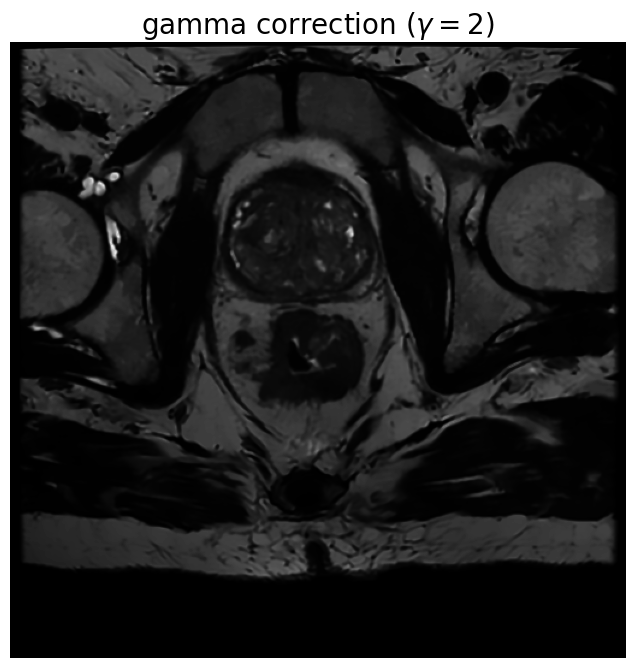
\includegraphics[width=.33\textwidth]{../images/gamma_2.png}\hfill
    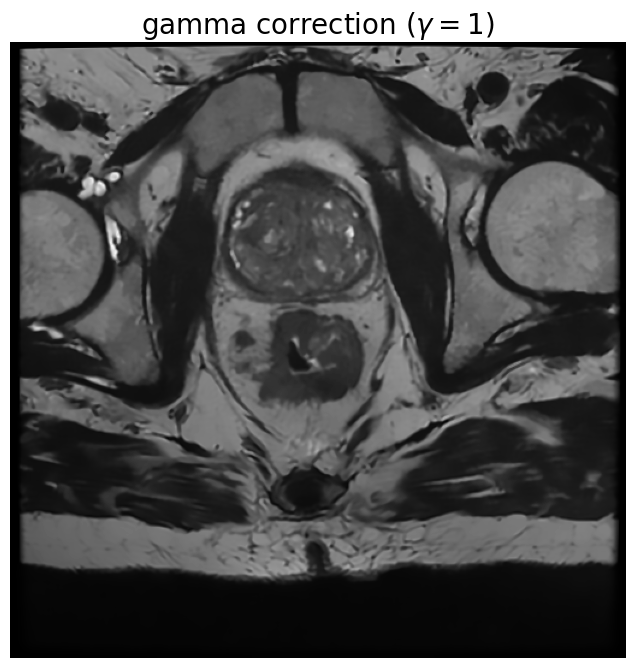
\includegraphics[width=.33\textwidth]{../images/gamma_1.png}\hfill
    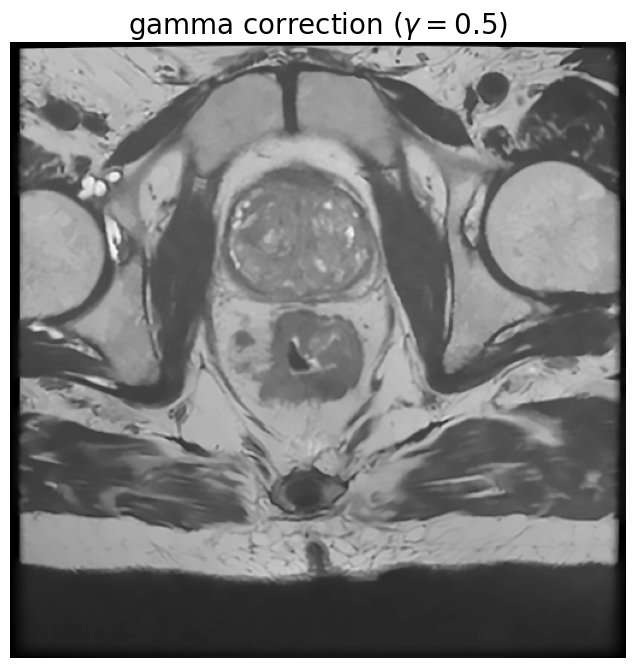
\includegraphics[width=.33\textwidth]{../images/gamma_1.5.png}
    
\caption{Example of gamma correction, applied to a MR image, varying $\gamma$.
As you can see, a value of $\gamma$ larger than 1 enhances darker regions while a value smaller than 1 makes dark regions lighter; a value of $\gamma$ equal to 1 corresponds to the original image.
Images from IRCCS Sant’Orsola-Malpighi Policlinic Dataset.}
    
\end{figure}

\end{document}

\newpage
    % SEGMENTATION
    \documentclass{standalone}
\usepackage{xr}
\externaldocument{../Chapter2/intro}
\begin{document}
\subsection{Segmentation}
Once trained, the CNN model was used for the segmentation of the MRI scans of each patient.
Before the segmentation, the scans are pre-processed as previously described.
\\
The segmentation is done slice by slice, for each patient, by using the trained CNN model to obtain the predicted tumor area.
The prediction values range between 0 and 1.
\\
Then, using \textsc{OpenCV}\cite{opencv_library} functions it is possible to obtain a segmented area like the one in Figure \ref{contoured}, where the red contour represents the border of the predicted tumor area.


\begin{figure}[htp]

    \centering
    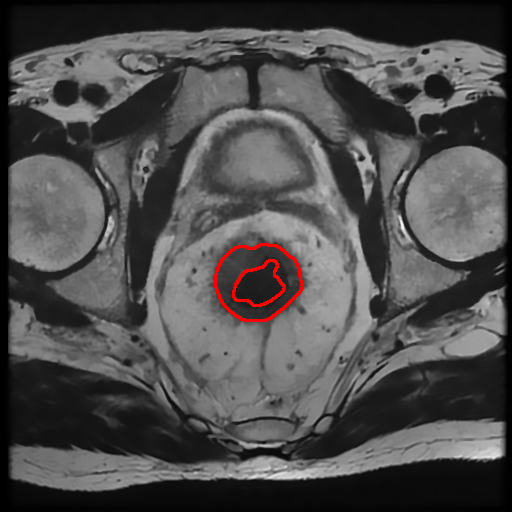
\includegraphics[width=.49\textwidth]{../images/BO56_9_cont.png}
    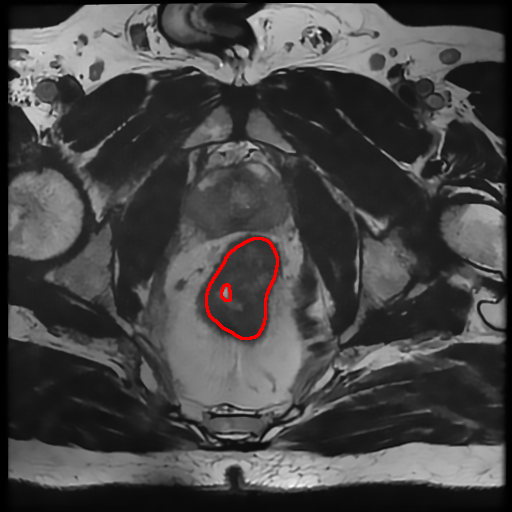
\includegraphics[width=.49\textwidth]{../images/BO85_6_cont.png}
    
    \caption{Images of colorectal cancer with identified tumor areas from two different patients. The red contour represents the border of the predicted tumor area.}
    \label{contoured}
    
    \end{figure}


\end{document}

        % METHODS
        \documentclass{standalone}
\begin{document}
\subsection{Methods}
During the year several segmentation methods have been developed\cite{biondi}.
There are several ways to classify these methods.
For example, depending if they require or not a training set of data, they can be classified into \textit{supervised} or \textit{unsupervised} methods.
More, they can be classified depending on the information type they use, like \textit{Pixel classification} methods, which use only information about pixel intensity, or \textit{Boundary following} methods which use edge information etc...\cite{biondi}.\\
Among the most common ones:

\paragraph{Thresholding}
is a very simple and common approach to segmentation.
This method is applied on the \textit{histogram} of the image.
The histogram of a digital image with intensity levels $L$ in the range $[0, \: L-1]$, is a discrete function $h(l_k) = n_k$ where $l_k$ is the k-th intensity value and $n_k$  is the number of pixels with intensity $l_k$.\\
Thresholding consists in binarizing an image through an (if) clause on the intensity value of each point after having determined a threshold value $T \in [0, \: L-1]$.
The threshold value $T$ is usually chosen by visual assessment on the image histogram but it can be automatize by algorithms like the \textit{Otsu algorithm}.
One drawback of this method is that some parts of the image can belong to the same class even if they belong to different objects.
In fact, thresholding does not take into account the spatial characteristics of the image.
Moreover, it is sensitive to noise and intensity inhomogeneity that corrupt the image histogram and make difficult the classification of pixels\cite{biondi}.

\begin{figure}[htp]

    \centering
    \includegraphics[width=.45\textwidth]{../images/thresholdhistogram.png}
    \includegraphics[width=.45\textwidth]{../images/thresholdexample.png}
    
    \caption{Example of thresholding segmentation using Fiji software\cite{Fiji}. \\
    \textit{ Left)} Image Histogram.\textit{ Right)} Result of thresholding.}
    \label{thresholding}
    
    \end{figure}


\paragraph{Artificial Neural Networks} 
are computational architectures derived from neural physiological models\cite{segmentationreview}.
Artificial Neural Networks (ANNs) have evolved into a broad family of techniques.
For visual analysis are usually used Convolutional Neural Networks (CNNs) based on \textit{convolution kernels} or \textit{filters} that slide along input data to extract feature maps\cite{wiki:cnn}.
Several architectures have been developed over the years, for different tasks and fields of application.
In bio-medical image processing, the so-called U-Net\cite{unet}, is one of the most common architecture.
U-Net is a kind of CNN which allows overcoming the requirement of many training data\cite{biondi, unet}.
However a better explanation of ANNs will be provided in the following chapter.




\end{document}
        
        % UNET
        \documentclass{standalone}
\begin{document}
\section{U-Net}
The U-net is a convolutional network architecture for fast and precise segmentation of images especially in the biomedical field\cite{unet}.
One of the main advantage of the U-net is the ability of dealing with small dataset. The name U-net refers to the U shape of the network architecture. 
The whole structure is divided into two main parts, as shown in Figure\ref{fig:unet}:

\paragraph{Encoder}:
or contraction path is a sequence of convolutional and max pooling layers with the aim of extracting features and reducing dimensionality.

\paragraph{Decoder}:
or expansion path is a sequence of transpose convolutional layers to with the aim of reconstruct the feature map and consequently the segmentation mask.
\begin{figure}[htp]

    \centering
    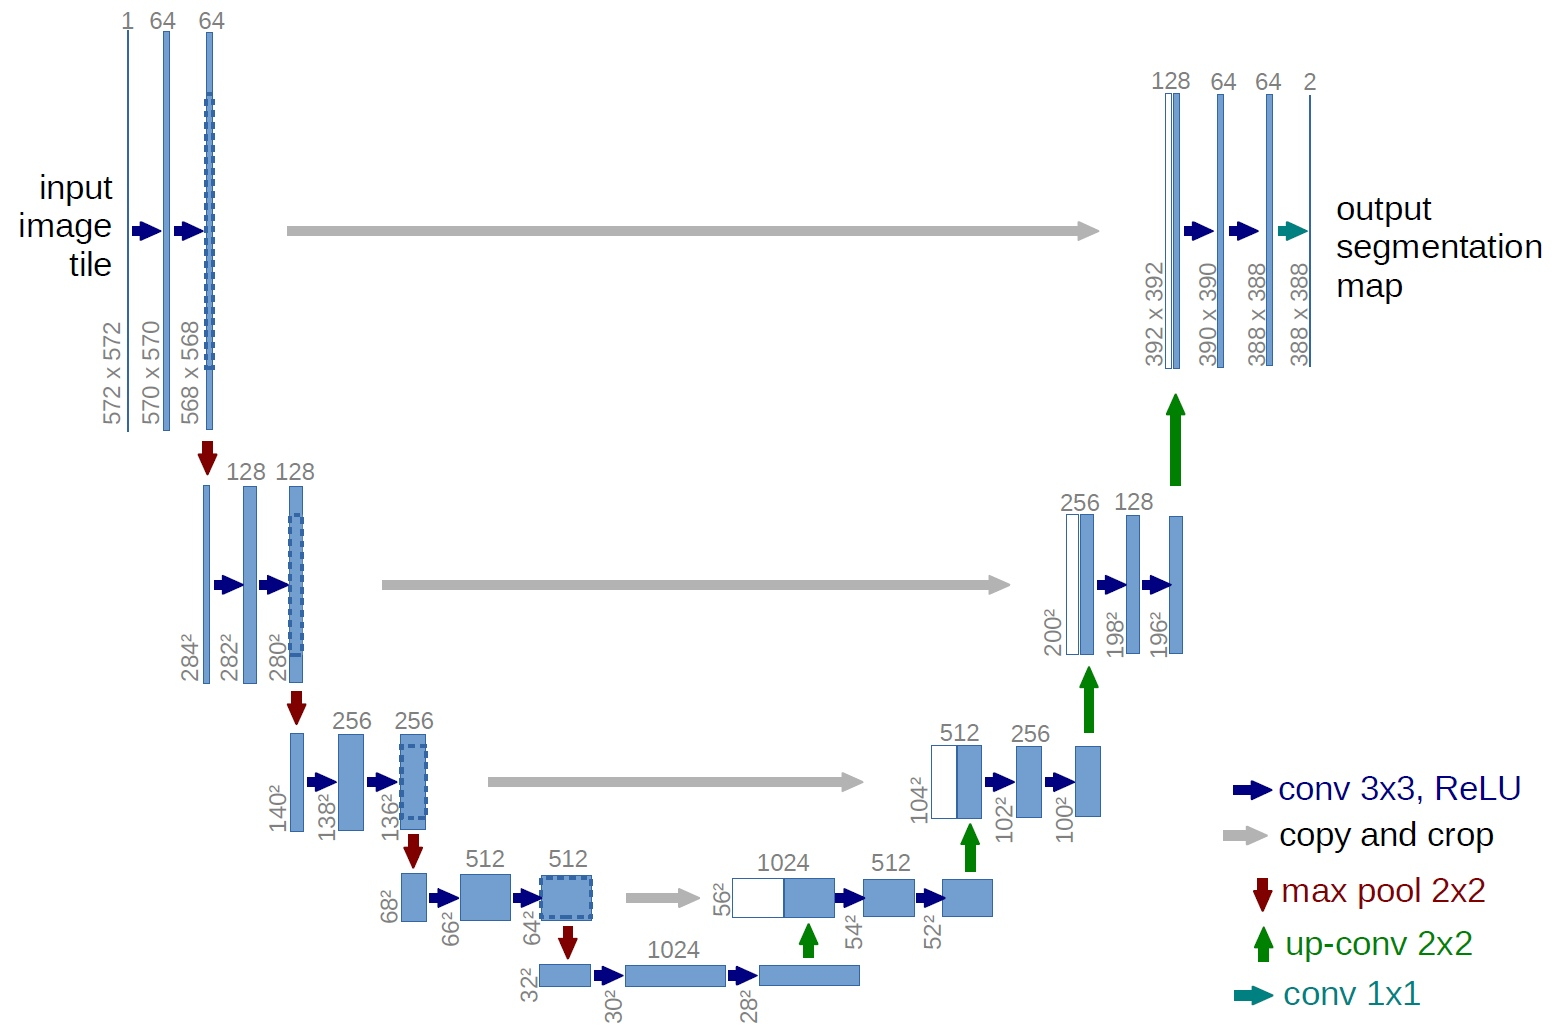
\includegraphics[width=.9\textwidth]{../images/U-Net arch.jpeg}
    
    \caption{Original U-Net architecture. From\cite{unet}}
    \label{fig:unet}
    
    \end{figure}
\\
The \textit{Encoder} is a typical Convolutional Neural Network that consists in the repeated application of convolutions, followed by ReLu activation function and max pooling operations.
During the contraction the input size is decreased and so the spatial information, while the information about features is increased.
The \textit{Decoder} combines the features extracted in the contraction path  with tha spatial information by a sequence of transpose convolutions (or up-convolutions) and concatenations (grey arrows in Figure\ref{fig:unet}).



\end{document}

\newpage
    % RADIOMICS
    \documentclass{standalone}
\begin{document}
\section{Radiomics}
Radiomics consists in methods that extract from medical images a large number of features, which have the potential to uncover disease characteristics that fail to be appreciated by the naked eye\cite{wiki:Radiomics}.
The main objective of radiomics is to assist the subjective interpretation of the clinicians with an objective prediction.
In the new era of precision medicine, radiomics is an emerging translational research field that aims to find associations between qualitative and quantitative information extracted from clinical images and clinical data to support the decision making process\cite{tesicoppola}.
Radiomic features can be divided into different classes:
\begin{itemize}
    \item First Order Statistics
    \item Shape based features 2D and 3D
    \item Gray Level Co-occurrence Matrix (GLCM)
    \item Gray Level Size Zone (GLSZM)
    \item Gray Level Run Length Matrix (GLRLM)
    \item Neighbouring Gray Tone Difference Matrix (NGTDM)
    \item Gray Level Dependence Matrix (GLDM)
\end{itemize}

\end{document}

        % POSSIBLE PURPOSES OF RADIOMICS
        \documentclass{standalone}
\begin{document}
\subsection{Possible Purposes Of Radiomics}

The possible applications of radiomics are based on a very wide range, from the prediction of clinical outcomes to the oncological diagnosis.
In this subsection, a brief overview of some general possible purposes will be given.
\subsubsection{Prediction of clinical outcomes} 
Radiomic features may be useful for predicting patient survival and describing intratumoral heterogeneity as demonstrated in a study by Aerts et al. \cite{Aerts}.
More, the usefulness of radiomics for predicting the immunotherapy response of patients with non-small cell lung cancer (NSCLC) using pretreatment CT and PET-CT images has been demonstrated by other studies\cite{tesicoppola}.
\subsubsection{Prediction of metastases}
Radiomic features can also predict the metastatic stage of tumors. 
For example, many radiomic features were identified as predictors of distant metastasis of lung adenocarcinoma in a study by Coroller et al.\cite{Coroller}.
They concluded that radiomic features may be useful in identifying patients at high risk of developing distant metastases, guiding clinicians in choosing the most effective treatment for individual patients.
\subsubsection{Prediction of physiological events}
Another possible application of radiomics analysis is the prediction of physiological events. 
Indeed, radiomics can be applied for the characterization and investigation of complex physiological events such as brain activity, which is usually studied with specific imaging techniques such as functional magnetic resonance ”fMRI”\cite{tesicoppola}. 


\end{document}

    \newpage
    % PCA
    \documentclass{standalone}
\begin{document}
\markboth{CHAPTER 1. MATERIALS AND METHODS}{1.5. PCA}
\section{Principal Component Analysis}
Principal component analysis (PCA) is a technique to reduce data dimensionality.
It replaces the $n$ original variables by a smaller number, $q$, of linear combinations, called principal components, of the original variables.
The application areas include data compression, image analysis, pattern recognition, regression and classification prediction\cite{PCA}.\\
The most common definition of PCA, due to Hotelling, states that for a set of observed data vectors 
$ \{ \mathbf{t}_{n} \}$, $n \in \{1, \dots, N \} $, the $q$ principal axes $\mathbf{w}_j$, $j \in \{ 1, \dots, q \} $ are those orthonormal axes onto which the retained variance under projection is maximal.
The vectors $\mathbf{w}_j$ are given by the $q$ dominant eigenvectors (i.e. those with the largest associated eigenvalues $\lambda$) of the sample covariance matrix $\mathbf{S} = \sum_{n}^{} ( \mathbf{t_n} - \mathbf{\bar{t}}) ( \mathbf{t_n} - \mathbf{\bar{t}})^T / N$ such that  $ \mathbf{S}\mathbf{w}_j = \lambda_j \mathbf{w_j}$ and where $\mathbf{\bar{t}}$ is the sample mean.
The vector $\mathbf{x}_{n} = \mathbf{W^T} (\mathbf{t_n} - \mathbf{\bar{t}})$, where $ \mathbf{W} = (\mathbf{w}_1 , \mathbf{w}_2 \dots \mathbf{w}_j)$ is thus a q-dimensional reduced representation of the observed vector $\mathbf{t}_{n}$ \cite{PCA}.
As we have mentioned, $\lambda_j$ is just the variance of each new feature dimension.
How to choose an appropriate $q$ depends on the Variance Contribution Rate  $\alpha_j = \lambda_j / \sum_{j}^{} \lambda_j $. 
This can be determined by looking at the cumulative explained variance ratio as a function of the number of components as shown in figure \ref{cumulativevr}.


\begin{figure}[ht]

    \centering
    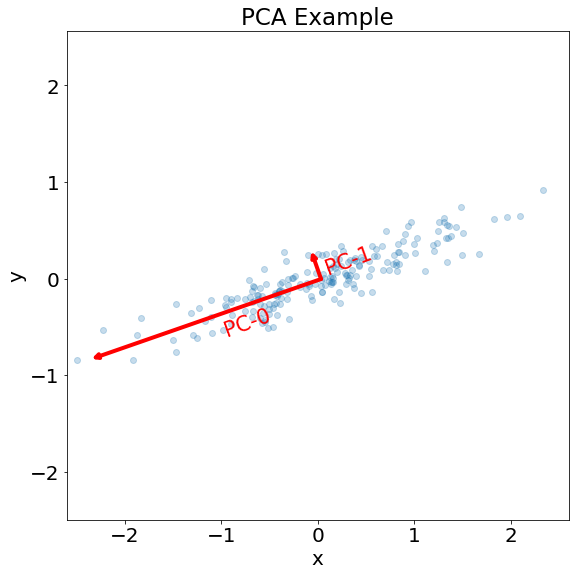
\includegraphics[width=0.62\textwidth]{../images/PCAexample1.png}
    
    \caption{Example of Principal Component Analysis.
     The red vectors represent the principal axes of the data, and the length of the vector is an indication of the variance of the data when projected onto that axis.}
    \label{PCAexample}
    
    \end{figure}

\markboth{CHAPTER 1. MATERIALS AND METHODS}{1.5. PCA}

\begin{figure}[htp]

    \centering
    \includegraphics[width=.68\textwidth]{../images/cumulative3.png}
    
    \caption{Example of cumulative explained variance ratio as a function of the number of components. This curve quantifies how much of the total variance is contained within the first N components. We can see that the first 10 components contain approximately $75 \%$ of the total variance, while to the reach the $100 \%$ you need around 50 components.}
    \label{cumulativevr}
    
    \end{figure}

\end{document}

    \newpage
    % SVC
    \documentclass{standalone}
\begin{document}
\markboth{CHAPTER 1. MATERIALS AND METHODS}{1.6. SVCs}
\section{Support Vector Classifiers}

Support Vector Classifiers (SVCs) are a subclass of Support Vector Machines (SVMs) that are a set of supervised learning methods (i.e. requires training data) used for purposes such as classification and regression.
A Support Vector Machine constructs a hyper-plane or set of hyper-planes in a high or infinite dimensional space.
Intuitively, a good separation is achieved by the hyper-plane that has the largest distance to the nearest training data points of any class (functional margin), since in general the larger the margin the lower the generalization error of the classifier\cite{SVCscikit, Bishop}.\\
For a SVC, mathematically, given training vectors $ \mathbf{x}_i \in \mathbb{R}^p ,  \: i \in \{1,\dots, n\} \:$, in two classes, and a vector $\mathbf{y} \in \{ -1, \: 1 \}^n$ (or $ \{0, \: 1 \}^n$), the goal is to find $\mathbf{w} \in \mathbb{R}^p$ and $b \in \mathbb{R}$ such that the prediction given by $sign(\mathbf{w^T  \mathbf{\Phi(x)}} + b)$ is correct for most samples \cite{SVCscikit}.\\
The function $\Phi(x)$ provides a convenient way of extending the analysis from the input space to a non-linear feature space by using a high-dimensional mapping. 
Finding a linear separating hyperplane in this feature space is equivalent to finding a non linear decision boundary in the input space\cite{SVCmapping}.\\
A SVC solves a primal problem and a dual problem. 
The primal:
\begin{equation}
    \min_{w, \zeta} \frac{1}{2} (\mathbf{w}^T  \mathbf{w}) + C \sum_{i = 1}^{n} \zeta_i
\end{equation}

subject to: $\begin{cases}
    y_i \cdot (\mathbf{w}^T  \mathbf{\Phi(x_i)} + b)  \geq 1 - \zeta_i, \\
    \zeta_i \geq 0 \quad i = 1, \dots, n 
    \end{cases}$
\newline
\\
\\
From an intuitive point of view, the minimization ($\mathbf{w}^T  \mathbf{w}$) corresponds to maximize the functional margin while incurring a penalty when a sample is misclassified or within the margin boundary.
The penalty term C controls the strength of this penalty, and acts as an inverse regularization parameter\cite{SVCscikit}.
Ideally, the term $\zeta_i$ should be 0 for a perfect prediction but real data are usually not always perfectly separable with a hyperplane, so some samples will be at a distance $\zeta_i$ from their correct margin boundary.
\\
The dual problem instead:
\begin{equation}
    \min_{\alpha} \frac{1}{2} (\mathbf{a}^T \mathbf{Q} \mathbf{a}) - \mathbf{e}^T \mathbf{a}
\end{equation}

subject to: $\begin{cases}
    \mathbf{y}^T \mathbf{a} = 0, &  \\
    0 \leq a_i \leq C  &  i = 1, \dots, n
    \end{cases}$
\newline
where $\mathbf{e}$ is the vector of all ones, $\mathbf{Q}$ is a $n \times n$ matrix: $Q_{ij}\equiv y_i y_j K(\mathbf{x_i}, \mathbf{x_j})$ where $K(\mathbf{x_i}, \mathbf{x_j}) = \mathbf{\Phi(x_i)}^T \mathbf{\Phi(x_j)} $ is the so called \textit{kernel}.
The $a_i$ terms are called \textit{dual coefficients}, and they are upper-bounded by C.\\


\newpage
\markboth{CHAPTER 1. MATERIALS AND METHODS}{1.6. SVCs}
Once these problems are solved, for a sample $\mathbf{z}$, the decision function is given by: 
\begin{equation}
    \sum_{i \in SV}^{}  y_i a_i \mathbf{K(x_i, z)} + b
\end{equation}
where the sum is over the supported  vectors (SV) that are the samples that lie within the margin because the dual coefficients $a_i$ are zero for the other samples\cite{SVCscikit}.

\begin{figure}[ht]

    \centering
    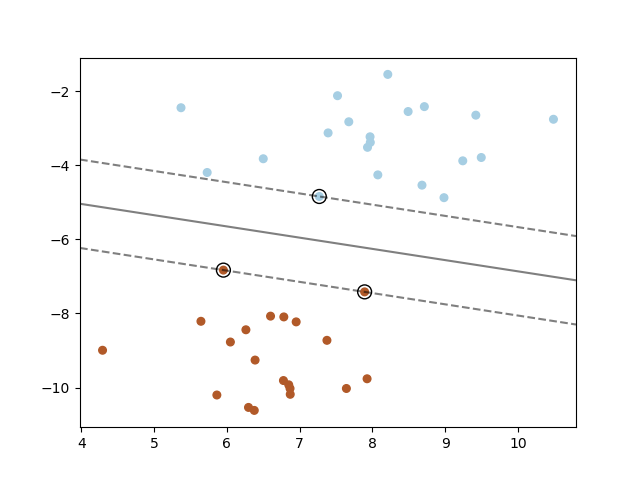
\includegraphics[width=.95\textwidth]{../images/svcexample.png}
    
    \caption{Classification made by a Support Vector Classifier (SVC) for a linearly separable problem. The gray line represents the line of the separation hyper-plane. The three samples on the margin boundaries (dashed lines) are called \textit{support vectors}. From \cite{SVCscikit}}\label{fig:svc}
    
    
    \end{figure}

\end{document}

    \newpage
    % METRICS
    \documentclass{standalone}
\begin{document}
\markboth{CHAPTER 1. MATERIALS AND METHODS}{1.7. METRICS}
\section{Performance Evaluation Metrics}

Performance evaluation metrics refer to a series of methods used to measure the performance of the developed pipeline.
This section is aimed at their definition.
\subsubsection{Precision}

The precision is the ratio between true positives $tp$ and the sum between true positives $tp$ with false positives $fp$.
The precision is intuitively the ability of the classifier to label not as positive a sample that is negative.
The best value is 1 and the worst value is 0.

\begin{equation*}
    Precision = \frac{tp}{tp + fp}
\end{equation*}


\subsubsection{Recall}

The recall is the ratio between true positives $tp$ and the sum between true positives $tp$ with false negatives $fn$.
The recall is intuitively the ability of the classifier to find all the positive samples.
The best value is 1 and the worst value is 0.

\begin{equation*}
    Recall = \frac{tp}{tp + fn}
\end{equation*}


\subsubsection{Dice Similarity Coefficient}
The Dice Similarity Coefficient or Dice-Sørensen coefficient (DSC) is a widely used metric in computer vision community to calculate the similarity between two images\cite{diceloss}.
Given two sets, X and Y, it is defined as:

\begin{equation*}
    DSC = 2 \cdot \frac{\mid  X \cap  Y \mid }{\mid X \mid + \mid  Y \mid }
\end{equation*}
where $\mid X \mid $ and  $\mid  Y \mid$  are the cardinalities of the two sets (i.e. the number of elements in each set). 
\\
Using the definition of true positive $tp$, false positive $fp$, and false negative $fn$, it can be written as:

\begin{equation*}
    DSC = \frac{2 tp}{2tp + fp + fn}
\end{equation*}
The best value is 1, meaning a perfect overlap between the two sets (i.e. ground-truth and predicted), while the worst value is 0 meaning no overlap.
\\
The Dice Similarity Coefficient is also known as F1-Score, and using the definition of \textit{precision} and \textit{recall} can be written as:

\begin{equation*}
    F1 = 2 \cdot \frac{precision \times recall}{precision + recall}
\end{equation*}

\markboth{CHAPTER 1. MATERIALS AND METHODS}{1.7. METRICS}

\subsubsection{Matthews correlation coefficient}
The Matthews correlation coefficient (MCC) is a measure of the quality of binary (two-class) classifications.
The MCC is a correlation coefficient ranging between -1 and +1. 
A coefficient of +1 represents a perfect prediction, 0 is an average random prediction, and -1 is an inverse prediction.
The MCC, using the definition of true positive $tp$, false positive $fp$, true negatives $tn$, and false negative $fn$,can be calculated by:

\begin{equation*}
    MCC = \frac{tp \times tn - fp \times fn}{ \sqrt{(tp + fp)(tp + fn)(tn + fp)(tn + fn)}}
\end{equation*}


\subsubsection{Confusion Matrix}

The Confusion Matrix is a specific table that allows visualization of the performance of an algorithm.
Each row of the matrix represents the instances in an actual class while each column represents the instances in a predicted class.
The diagonal elements represent the number of points for which the predicted label is equal to the true label, while off-diagonal elements are those that are mislabeled by the classifier. 

\subsubsection{Receiver Operating Characteristic curve}

The Receiver Operating Characteristic curve, or ROC curve is created by plotting the true positive rate (TPR) against the false positive rate (FPR).
By analyzing the ROC curves, the ability of the classifier to discern, for example, between a set A and B of population, is assessed, calculating the area under the ROC curve (AUC). 
The AUC value, between 0 and 1, is equivalent to the probability that a classifier will rank a randomly chosen positive instance higher than a randomly chosen negative one.
The ROC curves pass through the points (0,0) and (1,1), (0,1) and (1,1) represent two limit curves:
\begin{itemize}
    \item The first cuts the graph at $45$ degrees, representing the case of the random classifier ("no benefit" line), with the AUC equal to 0.5.
    \item The second curve is represented by the segment that from the origin rises to the point (0,1) and by the one that connects the point (0,1) to (1,1), having the AUC equal to 1, meaning a perfect classifier.
\end{itemize}

\end{document}

\end{document}